\section{Конструкторский раздел}
В данном разделе приведено описание структуры алгоритма и отдельных его этапов.
Представлена архитектура разрабатываемого программного продукта.
Продемонстрирована диаграмма класов, использующихся в работе

\subsection{Yake}
Общая структура работы алгоритма по извлечению ключевых слов представлена на рисунках \ref{fig:01a0} - \ref{fig:02a0}


\begin{figure}[!h]
	\centering
	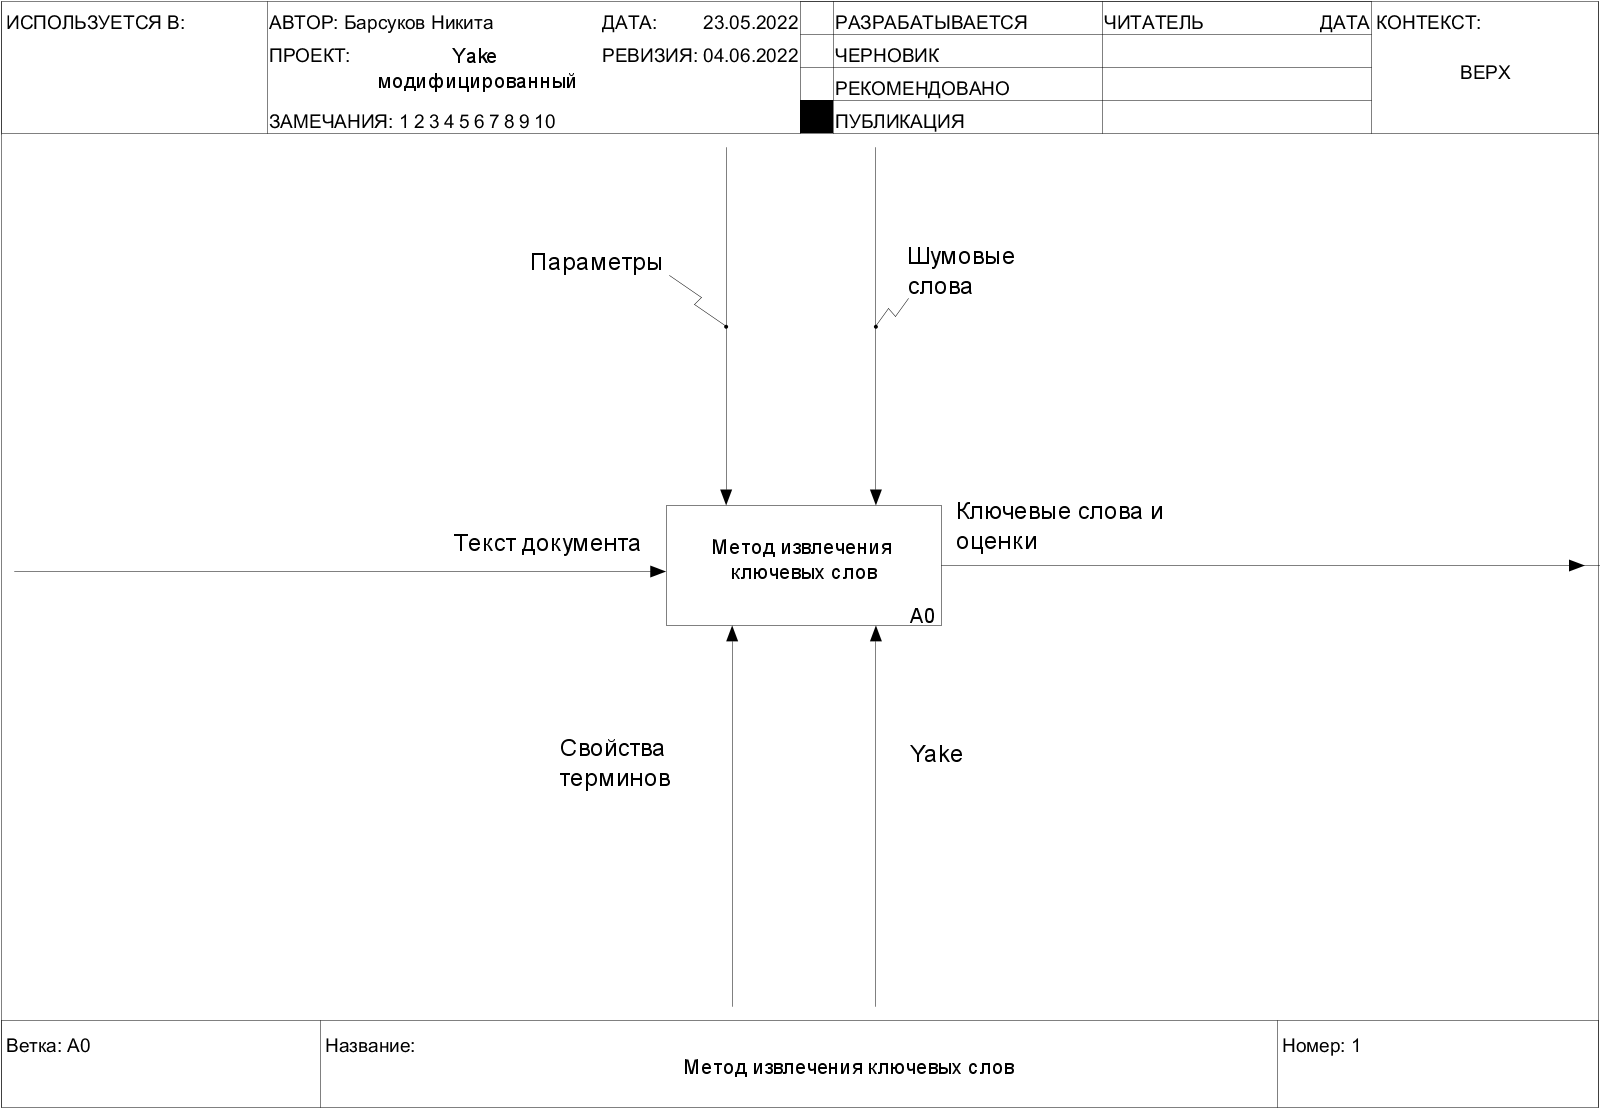
\includegraphics[width=1\linewidth]{src/img/idef0/Yake/01_A0}
	\caption{IDEF0 диаграмма разрабатываемого метода}
	\label{fig:01a0}
\end{figure}
Входными параметрами данного алгоритма являются тест извлеченный из электронного докумета и язык текста.
Резузьтатом исполнения данного метода является список, состоящий из кортежей, содержащих в себе термин и его оценку.

Данный метод можно разделить на несколько основных этапов, которые представлены на IDEF0-диаграмме, изображенной на рисунке \ref{fig:02a0}
\begin{figure}[!h]
	\centering
	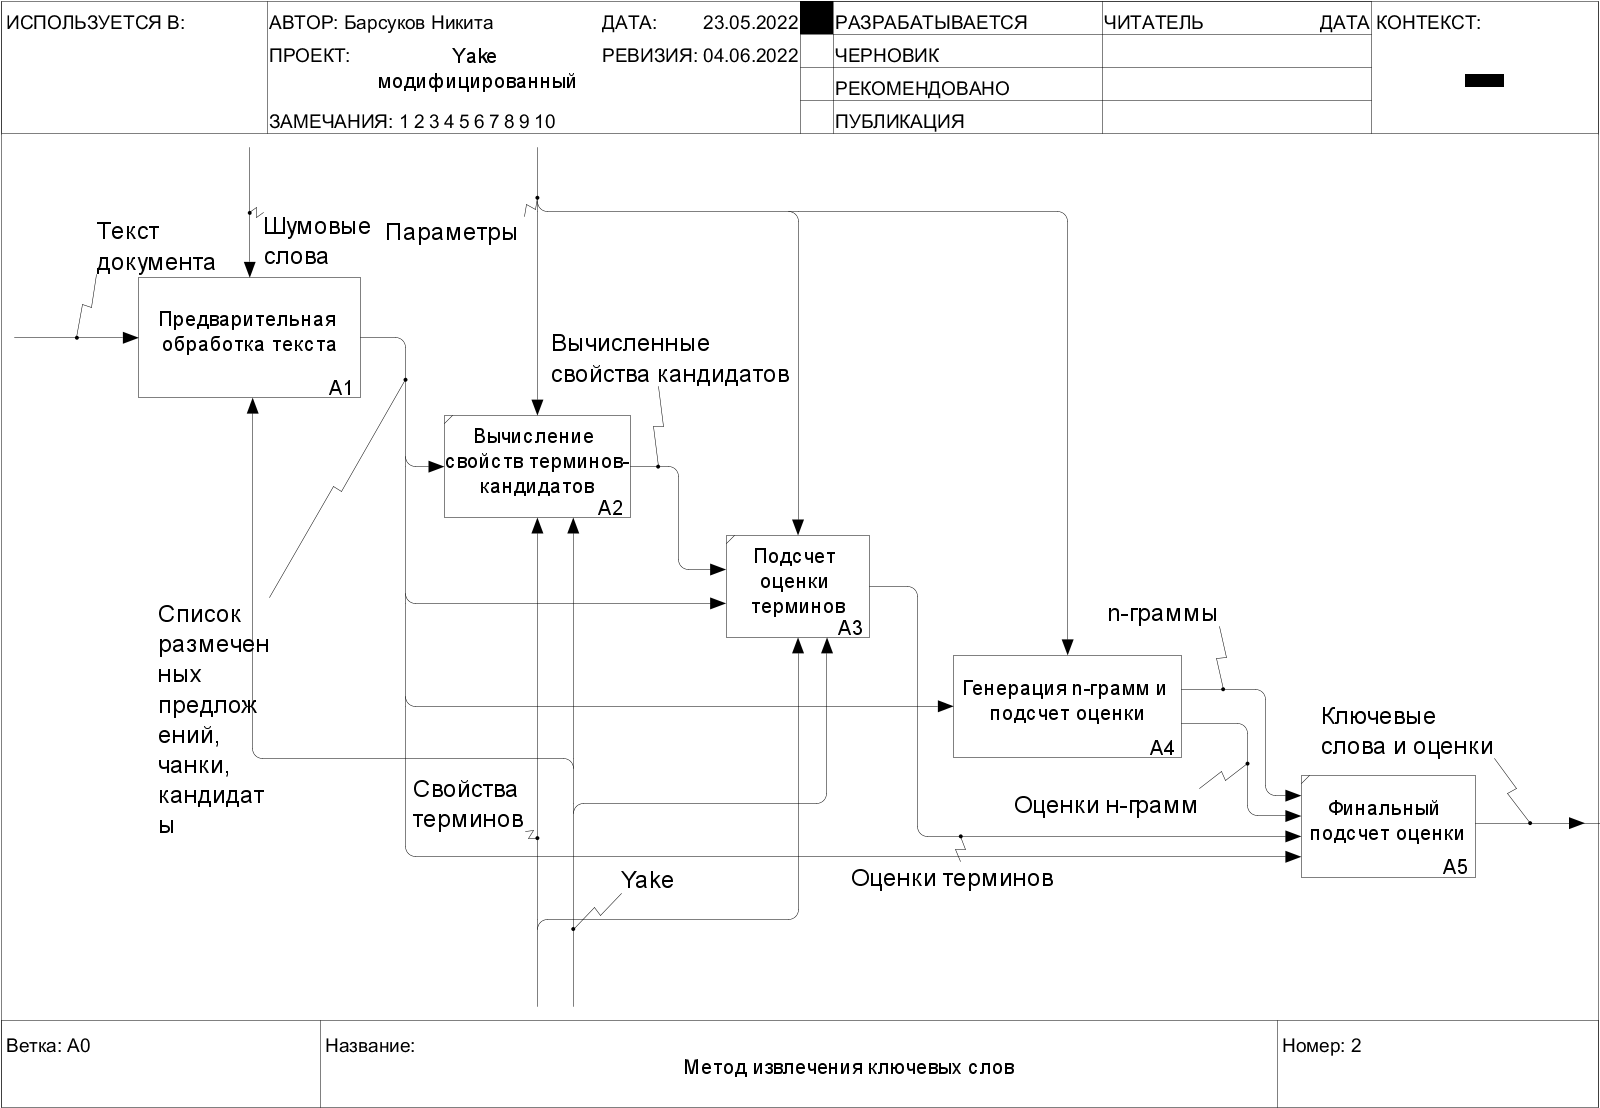
\includegraphics[width=1\linewidth]{src/img/idef0/Yake/02_A0}
	\caption{IDEF0 диаграмма модуля извлечения ключевых слов из текста}
	\label{fig:02a0}
\end{figure}

\begin{enumerate}
	\item предварительная обработка текста и выделение кандидатов (рисунок \ref{fig:02a0} блок А1)
	\item вычисление свойств термин-кандидатов (рисунок \ref{fig:02a0} блок А2)
	\item подсчет оценки кадидатов (рисунок \ref{fig:02a0} блок А3)
	\item генерация н-грамм и подсчет оценки (рисунок \ref{fig:02a0} блок А4)
	\item подсчет финальной оценки терминов (рисунок \ref{fig:02a0} блок А5)
\end{enumerate}

\subsection{Арихтектура ПО}
Для реализации программного обеспечения была выбрана MVC архитектура, разбивающая программу на три отдельных компоненты:
\begin{enumerate}
	\item представление - это отображение состояния внутренний системы;
	\item модель - это компонента отвечающая за предоставление данных конкретным элементам систмы;
	\item контроллер - это связующее звено между представлением и моделью, обрабатывает действия пользоватя, полученные от представления и отдает команды модели.
\end{enumerate}

Через графический интерфейс у пользователю должна быть возможность взаимодействия с программный ПО. 
Под взаимодействием подразумевается запуск ПО и получения результата.
Предоставляющийся функционал:
\begin{enumerate}
	\item выбор из списка методов извелечения КС от одного до нескольких алгоритмов;
	\item выбор одного или нескольких файлов через специальное окно;
	\item установка параметров для методов в отдельном окне;
	\item возможность ввести отдельно текстовую информацию.
\end{enumerate}

На рисунке \ref{fig:classdiagram} схематично отображены основные классы разрабатываемого программного продукта

Класс MainWindow - это входная точка приложения.
Он выполняет основную логику, связанную с обработкой пользовательский запросов к графическому интрефейсу.
Он взаимодействует с классом MethodControler, отвечающего за подгрузку, подготовку методов к работе.

\begin{figure}[!h]
	\centering
	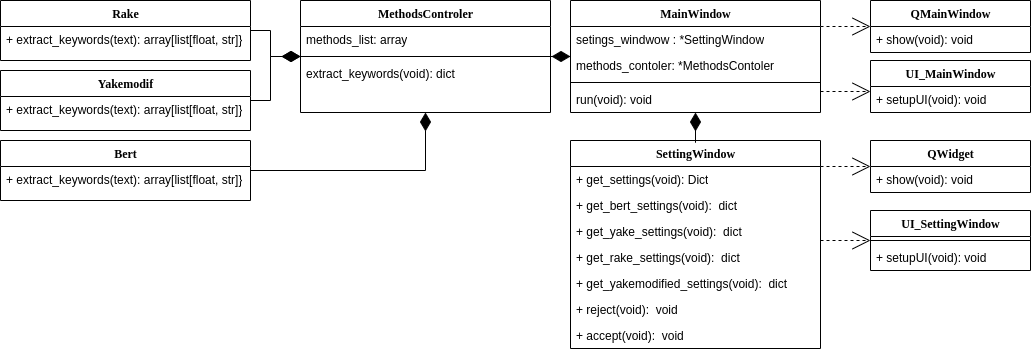
\includegraphics[width=1\linewidth]{src/img/class_diagram}
	\caption{Схематическое представление архитектуры программного обеспечения}
	\label{fig:classdiagram}
\end{figure}

